\newcommand{\Morph}{u}

\chapter{Computational aspects}

\section{Systems of chemical reactions}
Reaction-diffusion equations are an idealized and abstract representation of reality. They capture two phenomena, chemical reactions and diffusion. Mathematically, this is represented as a system of partial differential equations (PDEs), whose numerical solution requires discretization of time and space. Computation of the chemical reactions at a specific point in space depends on the elapsed time and previous concentration. Computation of diffusion, however, depends additionally on the concentrations in the areas adjacent to the point of interest.

\section{Isotropic Diffusion}
Diffusion is a process in which particles of a substance move from areas with high concentration to areas with low concentration. This change in concentration over space is referred to as a gradient. Diffusion was formalized in 1855 by Fick's second law:
\begin{equation}
\label{eq:ficks2ndlaw0}
	\frac{\partial \Morph}{\partial t} = \Div (D \nabla \Morph).
\end{equation}
$\Div$ is the divergence operator, $\nabla$ is the gradient operator, and $\Morph$ is a scalar field. Given Eqn. \ref{eq:ficks2ndlaw0}, we see that the diffusion rate depends on the gradient of the concentration. At a given location, the divergence of the gradient of $\Morph$ measures the difference between the concentration at that point and the average of the neighbouring concentrations. Diffusion is proportional to this change in concentration. However, particle size and domain porosity also affect the diffusion rate. This is represented by the diffusivity coefficient $D$. If diffusivity is the same regardless of direction, this diffusion is said to be isotropic, and we can simplify Eqn. \ref{eq:ficks2ndlaw0} to:
\begin{equation}
\label{eq:ficks2ndlaw1}
	\frac{\partial \Morph}{\partial t} = D \Lap \Morph.
\end{equation}
$\Lap$ is the divergence of the gradient and is called the Laplacian. Formally, it is the sum of the second spatial derivative in each basis direction $x_i$.
\begin{equation}
\label{eq:laplacian}
	\Lap = \sum_{i=0}^{n} \frac{\partial^2}{\partial x_i^2}.
\end{equation}
	
\section{Anisotropic diffusion}
In many biological scenarios, particles do not diffuse at an equal rate in all directions. In that case, the diffusion is called anisotropic, and the diffusivity coefficient changes based on the direction considered. For anisotropic diffusion, a single scalar $D$ no longer suffices. We can represent anisotropy by a tensor $\Lambda$. In the two-dimensional case, the tensor has the form:
\begin{equation}
\label{eq:diffTensor}
\Lambda =
\begin{bmatrix}
    \lambda_1 & 0 \\
    0 & \lambda_2 
\end{bmatrix}
\end{equation}
Each $\lambda_i$ represents the diffusivity in a basis of the space. Thus, $\Lambda$ is axis-aligned. Arbitrary orientations can be calculated with a rotation matrix $R$, allowing us to represent general anisotropic diffusion:
\begin{equation}
\label{eq:anisoDiffTensor}
	D = R^T \Lambda R.
\end{equation}
Now we can use $D$ to transform the gradient and thereby the diffusion rate, obtaining Eqn. \ref{eq:ficks2ndlaw0}.

\section{Discrete diffusion operators}
To simulate reaction-diffusion, the domain on which it is simulated must be discretized, which in turn means that we must use a discrete version of the Laplacian.

\subsection{Diffusion on grids}
Grids of square cells are a common representation of domains. This has many benefits as grids are easy to represent, and the required differential operators are simple to implement. Each cell in the grid has an area associated with concentrations of morphogens. Computationally, concentrations are represented by a scalar value assigned to each cell.

\subsubsection*{Diffusion in 1D} 
Computing diffusion on a 1D grid of cells can be accomplished by representing the Laplacian through finite differencing operations. Because the Laplacian involves second-order derivatives, we can approximate it by computing the difference of two first-order differences for a grid cell centred at $\Morph_i$, where $i$ is the $i^{th}$ cell:
\begin{equation}
\begin{aligned} \label{eq:firstOrderDifference}
	T_0 &= \frac{(\Morph_{i} - \Morph_{i-1})}{h},\\
	T_1 &= \frac{(\Morph_{i+1} - \Morph_i)}{h}.
\end{aligned}
\end{equation}
Here $\Morph_{i-1}, \Morph_i, \Morph_{i+1}$ are morphogen concentrations at their respective grid cells, $T_0$ and $T_1$ are the first order differences, and $h$ is the distance between the centres of adjacent cells. The discrete Laplacian is then:
\begin{equation} 
\label{eq:secondOrderDifference}
	\Lap \Morph_i = \frac{T_1 - T_0}{h} = \frac{\Morph_{i-1} - 2\Morph_i + \Morph_{i+1}}{h^2}.
\end{equation}
This differencing can be represented as a convolution mask during computation, as shown below:
\begin{figure}[!ht]
\centering
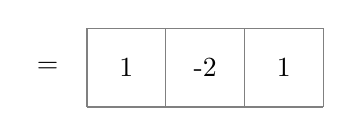
\begin{tikzpicture}
\draw[step=1.0cm,color=gray] (0,0) grid (3,1);
\node at (-0.5,+0.5) {$\Lap =$};
\node at (+0.5,+0.5) {1}; %\node at (+0.5, -0.25) {$f_{i-1}$};
\node at (+1.5,+0.5) {-2}; %\node at (+1.5, -0.25) {$f_i$};
\node at (+2.5,+0.5) {1}; %\node at (+2.5, -0.25) {$f_{i+1}$};
\end{tikzpicture}
\end{figure}	
	%\[\frac{\partial f_i}{\partial t} = \frac{\Lap*f}{h^2} \]
\subsubsection*{Diffusion in 2D}
In this case we have two directions to consider. Recall that the Laplacian is the sum of the second derivatives in each principle direction. This allows us to use the summation of the 1D case in both $x$ and $y$ directions, which, for a cell $\Morph_{i,j}$, yields:
\begin{equation} 
\label{eq:gridLaplacian}
	\Lap \Morph_{i,j} = \frac{\Morph_{i,j−1} + \Morph_{i,j+1} + \Morph_{i−1,j} + \Morph_{i+1,j} − 4\Morph_{i,j}}{h^2} .
\end{equation} 
Again, the Laplacian operator can be represented as a convolution mask:

\begin{figure}[H]
\centering
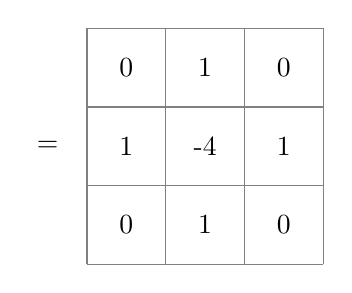
\begin{tikzpicture}
\draw[step=1.0cm,color=gray] (0,0) grid (3,3);
\node at (-0.5,+1.5) {$\Lap =$};
\node at (+0.5,+2.5) {0};
\node at (+1.5,+2.5) {1};
\node at (+2.5,+2.5) {0};
\node at (+0.5,+1.5) {1};
\node at (+1.5,+1.5) {-4};
\node at (+2.5,+1.5) {1};
\node at (+0.5,+0.5) {0};
\node at (+1.5,+0.5) {1};
\node at (+2.5,+0.5) {0};
\end{tikzpicture}
\end{figure}

\subsection{Diffusion on arbitrary triangular meshes}
Triangular meshes are ubiquitous in computer graphics. Meshes allow for a discrete representation of arbitrary surfaces, and there are well-studied algorithms for growing and subdividing them. These properties make meshes a good candidate for reaction-diffusion simulations. As in the grid case, concentrations are associated with cells. These cells are the faces of the mesh dual graph. Concentrations are stored at the vertices because each vertex is located at the centre of its cell. To allow for easy neighbour identification and area calculation, I represent the mesh as a half-edge data structure \citep{marschner2015}.

\begin{figure}[H]
    \centering
    \incfig{halfEdgeMesh}
    \caption{Two triangles and their half-edge representation denoted by black arrows.}
    \label{fig:halfEdgeMesh}
\end{figure}
Two half-edges replace each edge in the mesh to build this data structure. A single half-edge has a pointer to the next half-edge in the same face, as shown in Fig. \ref{fig:halfEdgeMesh}. Also, it has a pointer to the vertex that it originates from and a pointer to the complementary half-edge. Each vertex stores a scalar representing the area of the dual cell. This area is the sum of one-third of each adjacent face's area. %Alternate area partitions are given in \citep{Meyer2003}.

\subsubsection*{Isotropic diffusion on meshes}
To compute diffusion on an arbitrary triangular mesh, we need a discrete Laplacian. This Laplacian can be a generalization of Eqn. \ref{eq:gridLaplacian}:
\begin{equation}
(\Lap{} \Morph)_i = \frac{1}{A} \sum_{i \sim j} w_{ij}(\Morph_i - \Morph_j).
\end{equation}
This equation states that the Laplacian at vertex $i$ of the scalar field $\Morph$ is the sum of the weighted differences between the concentration at $i$, $\Morph_i$, and each neighbouring concentrations $\Morph_j$. The weight is $w_{ij}$, each edge is denoted $i \sim j$, and the area associated with $i$ is $A$. The choice of weight determines the behaviour of the discrete Laplacian. \citet{wardetzky2007} have shown that no discretization maintains all the properties of the continuous Laplacian. The most common weighting used is the cotangent Laplacian,
\begin{equation}
	(\Lap{} \Morph)_i = \frac{1}{2A} \sum_{i \sim j} (\cot{\alpha} + \cot{\beta)} (\Morph_i - \Morph_j).
	\label{eq:cotanLaplacian}
\end{equation}

A vertex $i$ and a neighbouring vertex $j$ are connected by an edge coloured black in Fig. \ref{fig:dualMesh}. The cotangent weight for the black edge is computed from the angles $\alpha$ and $\beta$, which are opposite from the edge. This weight can be derived from the ratio of the edge length of the dual cell, shown in red, and the black edge's length. The black edge length is inversely proportional to the magnitude of the morphogen gradient between $i$ and $j$. The length of the red edge represents how much of an interface between the area associated with $i$ and the area associated with $j$ exists. Consequently, the amount of diffusion increases when the length of the red edge increases. To find the cotangent Laplacian for the entire mesh, we evaluate Eqn. \ref{eq:cotanLaplacian} at each vertex. A rigorous derivation is given in \citep{crane2013, herholz2013}. The drawback of this Laplacian compared to the continuous version, is that the cotangent weights can be negative. This occurs when angles are greater than $90^\circ$. Consequently, care must be taken when meshing the domain.

\begin{figure}[H]
	\centering
	\incfig{dualMesh}
	\caption{A vertex $i$ and its dual area $A$. The weighting for the cotangent Laplacian between vertex $i$ and $j$ is dependant on the length of the red and black edges.}
	\label{fig:dualMesh}
\end{figure}

\subsubsection*{Anisotropic diffusion on meshes}

% 1. Pose the problem first in the context of a figure. 
%		Figure needs diffusion dir
% 2. Be as explanatory as possible
% 3. Introduce significant elements that come into play

Computing anisotropic diffusion on a mesh requires Laplacian weights that reflect the change in diffusivity for a given direction. The diffusivity at a vertex is represented by a diffusion tensor, $\Lambda$ (Eqn. \ref{eq:diffTensor}). The tensor can be visualized as an ellipse as shown in Fig. \ref{fig:anisoMesh}a. To properly orient $\Lambda$, we need a direction and normal vector to construct the rotation matrix $R$ (Eqn. \ref{eq:anisoDiffTensor}). For a given vertex, $v_i$, a vector, $\boldsymbol{\vec{d_i}}$ is specified. This provides a notion of direction on the mesh. To calculate a direction on a given face, the angle weighted average of its vertex directions, $\boldsymbol{\vec{d_i}}$, $\boldsymbol{\vec{d_j}}$, and $\boldsymbol{\vec{d_k}}$, is computed and projected onto the face to obtain $\boldsymbol{\vec{d_{ijk}}}$ (Fig. \ref{fig:anisoMesh}b). $\boldsymbol{\vec{d_{ijk}}}$ is then used with the face normal to obtain $R$, and subsequently, $D$. $D$ is applied to the morphogen gradients existing on the faces adjacent to the cell. The vertex $j$ in Fig. \ref{fig:anisoMesh} has a morphogen gradient which is perpinducular to the edge $e_j$ \cite{}. To find the gradient direction we apply a $90^\circ$ rotation matrix, $Q$, about the face normal to $e_j$. To apply $D$ to $e_j$ we do $Q^TDQe_j$.

\begin{figure}[H]
	\centering
	\incfig{aniso_vec2}
	\caption{\textbf{a:} the diffusion tensor at a vertex. The green and red arrows are the first and second principle diffusion directions, respectively. \textbf{b:} A triangle with diffusion vectors at each vertex and the resulting face vector.}
	\label{fig:anisoMesh}
\end{figure}


% 4. Present the formula
% 5. Explain the remaining elements in the formula

% Set the stage: "Here we have this kind of setup, and this is the dominant direction of diffusion."
% Tensor can be represented as an ellipse
% 

%To simulate anisotropic diffusion on a triangular mesh, each vertex is assigned two diffusivity scalars and a diffusion direction vector. For each face adjacent to a given vertex, tensor $\Lambda$ is oriented with $R$. To construct $R$, the face normal and a face direction (an angle-weighted average of the vertex directions projected onto the face) are used. $D$ is now used to transform the morphogen gradient on each face. From this we can build a matrix, $L$, representing discrete anisotropic Laplacian operator:

\begin{equation} 
   L_{ij} =
   \begin{cases} 
      -\frac{1}{2A}\sum\limits_{t} \frac{D^\perp e_i}{\norm{e_i}} \cdot \frac{e_i}{\norm{e_i}}(\cot{\alpha}+\cot{\theta})  & i = j \\
      \frac{1}{2A}(\Gamma \frac{\cos{\gamma}}{\sin{\alpha}} + \Xi\frac{\cos{\xi}}{\sin{\beta}})   & i \sim j \\
      0 & otherwise
   \end{cases}
   \label{eq:anisoLaplacian}
\end{equation}
This matrix is used to compute diffusion when given a vector of morphogen concentrations, $u$, by:
\begin{equation}
	Lu = \Lap u.
\end{equation}
This Laplacian is more complicated than before, and a complete derivation is given in \citep{mathieu2014}. Again, $i$ and $j$ are vertices. $e_i$ and $e_j$ are edges, as shown in Fig. \ref{fig:meshLaplacian}. $D^\perp = Q^T D Q$ where $Q$ is a $90^\circ$ rotation matrix about the face normal. This rotation will be used to get a vector in the direction of a face gradient. The face gradient vector is then transformed by the diffusion tensor, $D$. The amount that this vector is transformed determines the amount of the anisotropy. 

$\Gamma = \frac{\norm{D^\perp e_j}}{\norm{e_j}}$ and $\gamma$ is the angle between $e_i$ and $D^\perp e_j$. Which ensures that if the $D^{\perp} = I$ then $\gamma = \alpha$ and we have regular isotropic diffusion. $\Xi$ and $\xi$ are the same quantities measured on the adjacent triangle with that triangle's $D$. 

\begin{figure}[H]
	\centering
	\incfig{meshLaplacian}
	\caption{Two triangles with their angles and edges associated with the anisotropic cotangent Laplacian.}
	\label{fig:meshLaplacian}
\end{figure}

\section{Boundary Conditions}
PDEs determine the state of the simulation inside the domain. The simulation interacts with the world outside the domain based on boundary conditions. These conditions are specified when computing the PDEs. The two most common boundary conditions are Dirichlet and Neumann. Dirichlet specifies the morphogen values directly at the boundary. This is useful for defining morphogen sources or sinks. Neumann specifies the rate of change of the morphogens across the boundary. \ProgramName{} uses Neumann with a value of zero by default. Alternatively, the user can specify Dirichlet conditions and a constant morphogen value to be used at the boundary. Dirichlet is implemented by not updating the concentrations at the boundary so they remain constant. This is equivalent to \Quotes{no-flux} boundary conditions. To specify Dirichlet boundary conditions, the time step at boundary vertices can be set 0. This freezes the concentrations found along the boundary.
%When computing the discrete Laplacian, a boundary edge will have only one adjacent face. The missing angle is assumed to be 0.

=== needs work? ===

\section{Systems with dynamic structure}
In nature, domains grow over time, which can have an appreciable effect on pattern formation. One of them is a diluting effect on chemical concentrations that make up a pattern. When simulating directly on meshes, the face's area represents a minimum size of pattern detail that can be represented. Thus, it is important to consider the increase in face size from growth. To address this, a subdivision algorithm is used to split large triangles into a few smaller ones. Subdividing every face in the mesh can lead to small triangles to be subdivided unnecessarily and the total number of triangles to increase quickly. This is a problem because the simulation performance decreases as the number of vertices increases. 

\begin{figure}[H]
	\centering
	\incfig{recursiveSubdiv}
	\caption{Subdividing a face, shown in red, using longest-edge bisection. \textbf{a:} subdivision starts with the red triangle. \textbf{b-d:} the progression of algorithm.} 
	\label{fig:recursiveSubdiv}
\end{figure}

Adaptive subdivision is a technique used to only subdivide triangles with an area larger than a given threshold. This approach allows all triangles to maintain a similar area and limits the unnecessary creation of triangles. The choice of adaptive subdivision algorithm used determines the shape of the generated triangles. The desired shape for triangles that comprise the mesh is equilateral. If a triangle exhibits large-angle deviations from $60^{\circ}$, it can pose a problem for the simulation. The number and magnitude of deviations in a mesh give an informal notion of mesh quality and affects the simulation. Depending on the angle, the cotangent weights can be negative or widely varying due to the behaviour of cotan around 0 and 180 degrees. Negative cotangent weights cause diffusion to move morphogens from low to high concentrations incorrectly \citep{wardetzky2007}. 

To obtain optimal incremental triangulation that tends to produce good quality triangles, we use longest-edge bisection \citep{rivara1998}. In this method, faces are only ever subdivided with respect to their longest edge. The red triangle in Fig. \ref{fig:recursiveSubdiv}a is too large and must be subdivided. In Fig. \ref{fig:recursiveSubdiv}b, the red triangle has been subdivided, but the new edge does not connect to an edge in the adjacent face. To solve this, we also subdivide the adjacent face along its longest edge. This may fix the issue, or it may cause another triangle to be missing an edge. We proceed by subdividing every face missing an edge in the same way until the mesh is triangular again. This process is shown in Fig. \ref{fig:recursiveSubdiv} and the algorithm is detailed in Algorithm \ref{alg:subdivisionAlgorithm}. 

Subdivision also requires the proper handling of concentrations. The concentration assigned to the new vertex is the average of the neighbouring concentration values that shared the edge.

\begin{algorithm}[!ht]
  \KwIn{Triangle t0}
  \KwResult{Triangle is subdivided along its longest edge. Adjacent triangles are recursively subdivided to share edges.}
  \SetKwFunction{subdivide}{subdivide}
  \SetKwProg{myalg}{}{}{}
  \myalg{\subdivide{Triangle t0}}
  {
   Edge \textit{e0 = getLongestEdge(t0)}\\
   bool \textit{subdividing = hasAdjacentFace(e0)}\\
   \textit{subdivideFace(t0, e0)}\\
   \While{subdividing}
   {
    \eIf{hasAdjacentFace(e0)}
    {
      Triangle \textit{t1 = getAdjacentFace(e0)}\\
      Edge \textit{e1 = getLongestEdge(t1)}\\
      \eIf{e1 == getPairEdge(e0)}
      {
       \textit{subdivideFace(t1, e1)}\\
       \textit{subdividing = false}\\
      }{
        \textit{subdivide(t1)}\\   
      }
    }{
     \textit{subdividing = false}\\
    }
   }
  }
  \textbf{end}
  \caption{An algorithm to recursively subdivide a triangle and its neighbours based on \citep{rivara1998}.}
  \label{alg:subdivisionAlgorithm}
\end{algorithm}

\section{Numerical methods}

The simulation is advanced by taking small steps through time from a given initial condition. I use the forward Euler method \citep{solomon2015} to perform this integration. A reaction-diffusion formula integrated with forward Euler is:
\begin{equation}
	\boldsymbol{x_{i+1}} = \boldsymbol{x_{i}} + (D\Lap{}\boldsymbol{x_i} + F(\boldsymbol{x_i}))\Delta t. \\
\end{equation}
Here $\boldsymbol{x_i}$ is a vector of scalars representing morphogen concentrations at step $i$ and $\Delta t$ is the time-step. $D$ is diffusivity, $\Lap{}$ is the discrete Laplacian used to compute diffusion, and $F(\boldsymbol{x_i})$ encapsulates the reactions of the system. This method suffers from inaccuracy at larger time-steps because we are assuming $\Lap{}\boldsymbol{x_i} + F(\boldsymbol{x_i})$ is constant for the whole time-step. This inaccuracy can cause instability in stiff equations by accruing error with each simulation step. Semi-implicit integration schemes \citep{Nie2006} allowing for larger time-steps, but in practice, it is possible to use small enough time-steps to minimize inaccuracy and avoid instability. 


